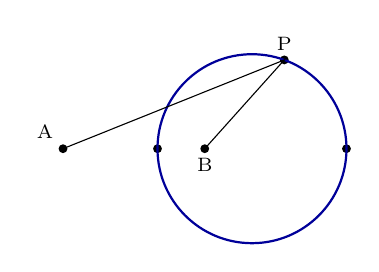
\begin{tikzpicture}[x=6mm,y=6mm]
\ax{-1}{7}{-2.6}{2.8}
\fill (0,0) circle (1.6pt);
\node[above left] at (0,0){\scriptsize A};
\fill (3,0) circle (1.6pt);
\node[below] at (3,0){\scriptsize B};
\fill (2,0) circle (1.6pt);
\fill (6,0) circle (1.6pt);
\fill (4.684040286651338,1.8793852415718166) circle (1.6pt);
\node[above] at (4.684040286651338,1.8793852415718166){\scriptsize P};
\draw[thick,blue!60!black] (4,0) circle (2);\draw (0,0)--(4.684,1.879)--(3,0);
\end{tikzpicture}